\section{The maximum stellar mass and cluster formation}
Assuming the stellar IMF is a continuous density distribution function and that
clusters are filled with stars distributed according to the stellar IMF, this can
be generalized by stating that each cluster can have only one most massive star,
\begin{equation}
1=\int_{m_{max}}^{m_{max*}}\xi(m')dm',
\end{equation}
with,
\begin{equation}
M_{ecl}(m_{max})=\int_{m_{low}}^{m_{max}} m' \xi(m')dm',
\end{equation}
as a further condition, as above. These two equations need to be solved numerically and give the semi-analytical relation $ m_{max}= \eta (M_{ecl} )$(Weidner & Kroupa
2004). It is plotted in figure \ref{fig:max-mecl}.
\begin{figure}
	\centering
	\begin{subfigure}[b]{0.4\textwidth}
%		\centering
		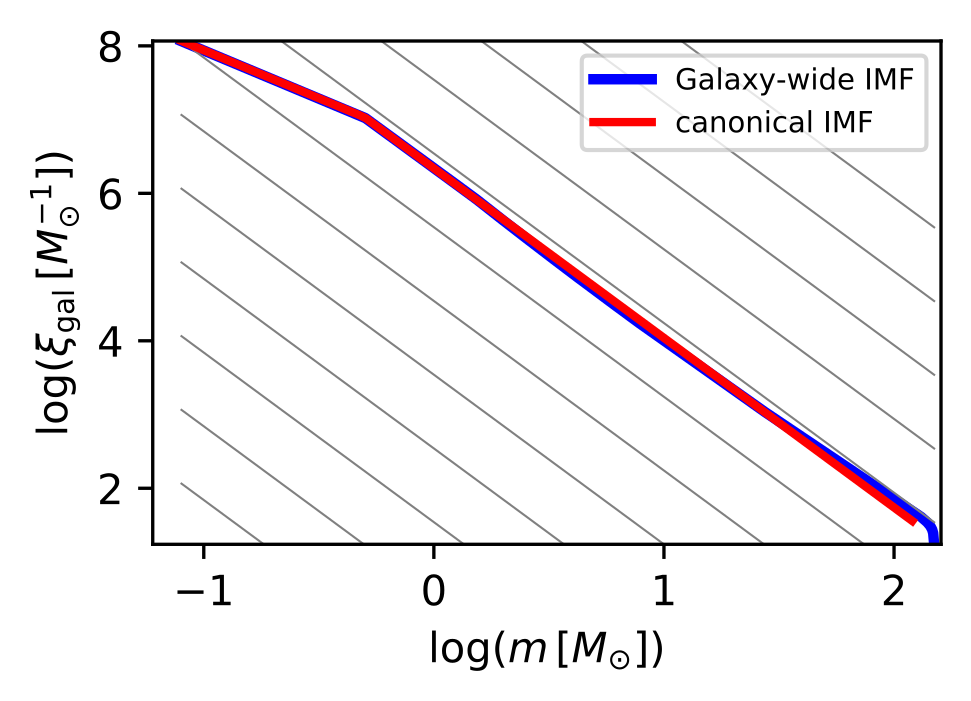
\includegraphics[width=\textwidth]{sfr1-feh0.png}
		\caption{SFR=1, $[\frac{Fe}{H}]=0$}
		\label{fig:2d-5dt}
	\end{subfigure}
	\begin{subfigure}[b]{0.4\textwidth}
	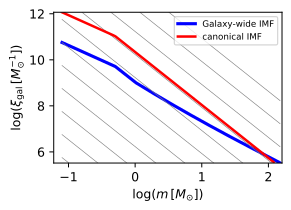
\includegraphics[width=\textwidth]{sfr1e4-feh0.png}
	\caption{SFR=$10^4$, $[\frac{Fe}{H}]=0$}
	\label{fig:2d-5dt}
	\end{subfigure}
	\begin{subfigure}[b]{0.45\textwidth}
%	\centering
	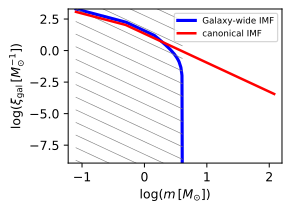
\includegraphics[width=\textwidth]{sfr1e-5-feh0.png}
	\caption{SFR=$10^{-5}$, $[\frac{Fe}{H}]=0$}
	\label{fig:2d-5dt}
	\end{subfigure}
	\caption{rebuild of A selection of IGIMF models which related to metalicity (in form of $[\frac{Fe}{H}$]=1,0,-3,-5)and SFR=$10^{-5},1,10^{4} \frac{M_{\odot}}{yr}$. All IMF models are
		normalized to the total stellar mass formed over $\delta t = 10 Myr$ to make the comparison with the canonical IMF (black dashed line in each panel)
		quantitative.}
	\label{fig:feh=0}
\end{figure}

\begin{figure}
	\centering
		\begin{subfigure}[b]{0.4\textwidth}
		%	\centering
		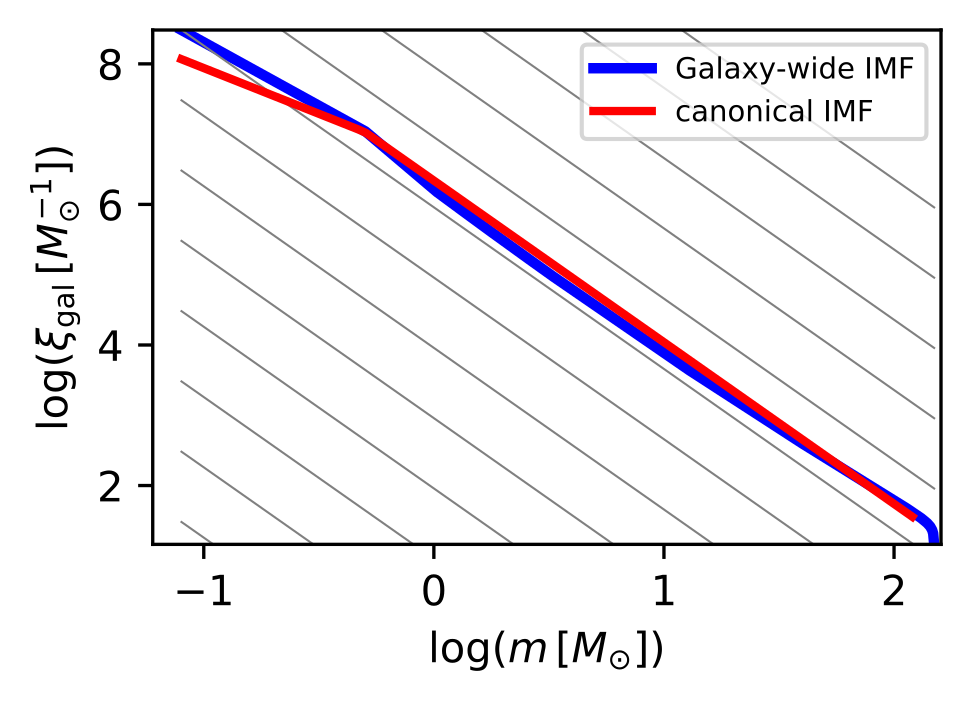
\includegraphics[width=\textwidth]{sfr1-feh1.png}
		\caption{SFR=$10^{0}$, $[\frac{Fe}{H}]=1$}
		\label{fig:s1e4-1}
	\end{subfigure}
	\begin{subfigure}[b]{0.4\textwidth}
		%	\centering
		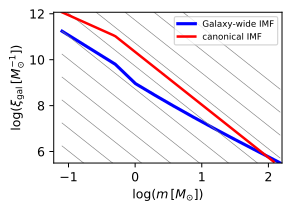
\includegraphics[width=\textwidth]{sfr1e4-feh1.png}
		\caption{SFR=$10^{4}$, $[\frac{Fe}{H}]=1$}
		\label{fig:s1e4-1}
	\end{subfigure}
\begin{subfigure}[b]{0.45\textwidth}
	%	\centering
	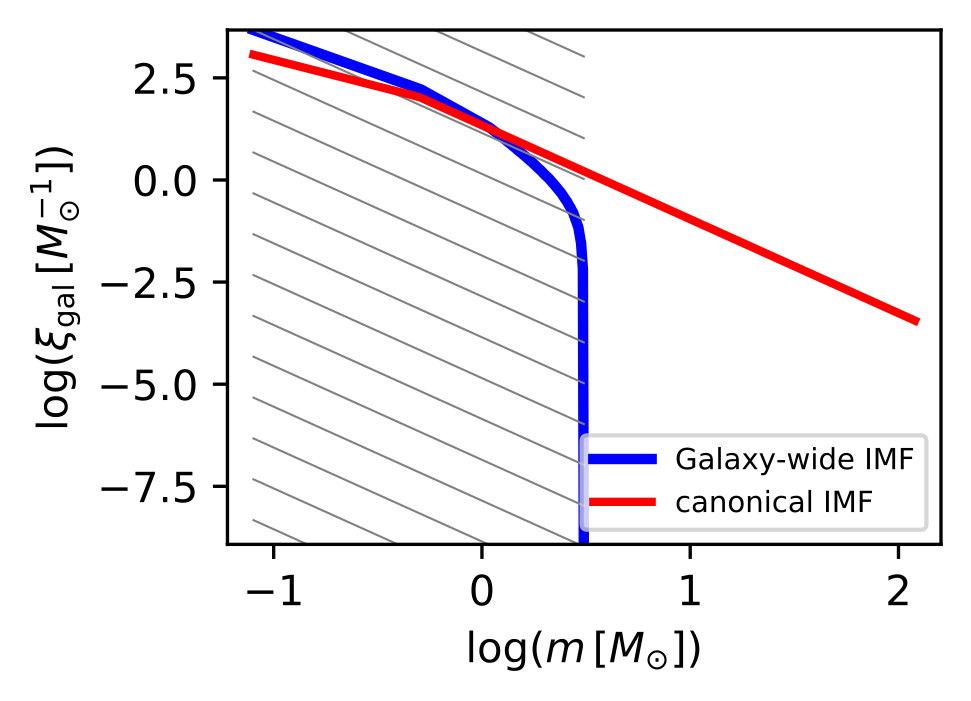
\includegraphics[width=\textwidth]{sfr1e-5-feh1.png}
	\caption{SFR=$10^{-5}$, $[\frac{Fe}{H}]=1$}
	\label{fig:s1e4-1}
\end{subfigure}
	\caption{rebuild of A selection of IGIMF models which related to metalicity (in form of $[\frac{Fe}{H}$]=1,0,-3,-5)and SFR=$10^{-5},1,10^{4} \frac{M_{\odot}}{yr}$. All IMF models are
	normalized to the total stellar mass formed over $\delta t = 10 Myr$ to make the comparison with the canonical IMF (black dashed line in each panel)
	quantitative.}
\label{fig:grid-sfr}
\end{figure}

\begin{figure}
	\centering
	\begin{subfigure}[b]{0.4\textwidth}
		%	\centering
		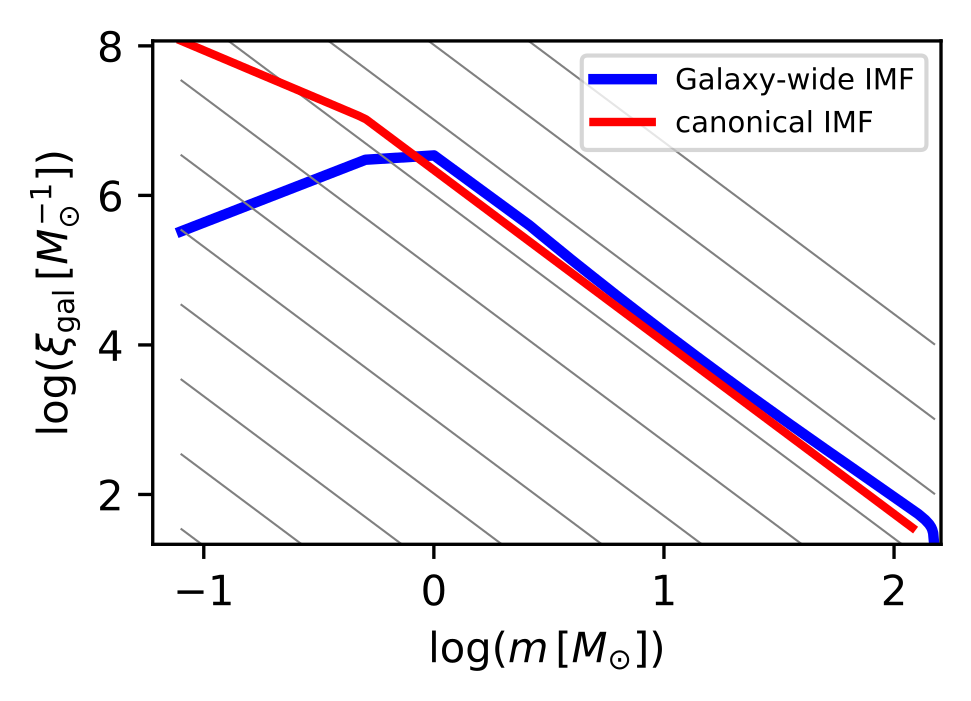
\includegraphics[width=\textwidth]{sfr1-feh-5.png}
		\caption{SFR=$10^{0}$, $[\frac{Fe}{H}]=-5$}
		\label{fig:s1e4-1}
	\end{subfigure}
	\begin{subfigure}[b]{0.4\textwidth}
		%\centering
		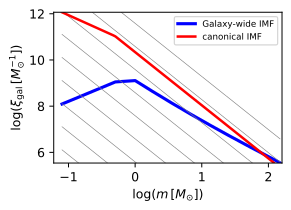
\includegraphics[width=\textwidth]{sfr1e4-feh-5.png}
		\caption{SFR=$10^{4}$, $[\frac{Fe}{H}]=-5$}
		\label{fig:2d-5dt}
	\end{subfigure}
	
	\begin{subfigure}[b]{0.45\textwidth}
		%\centering
		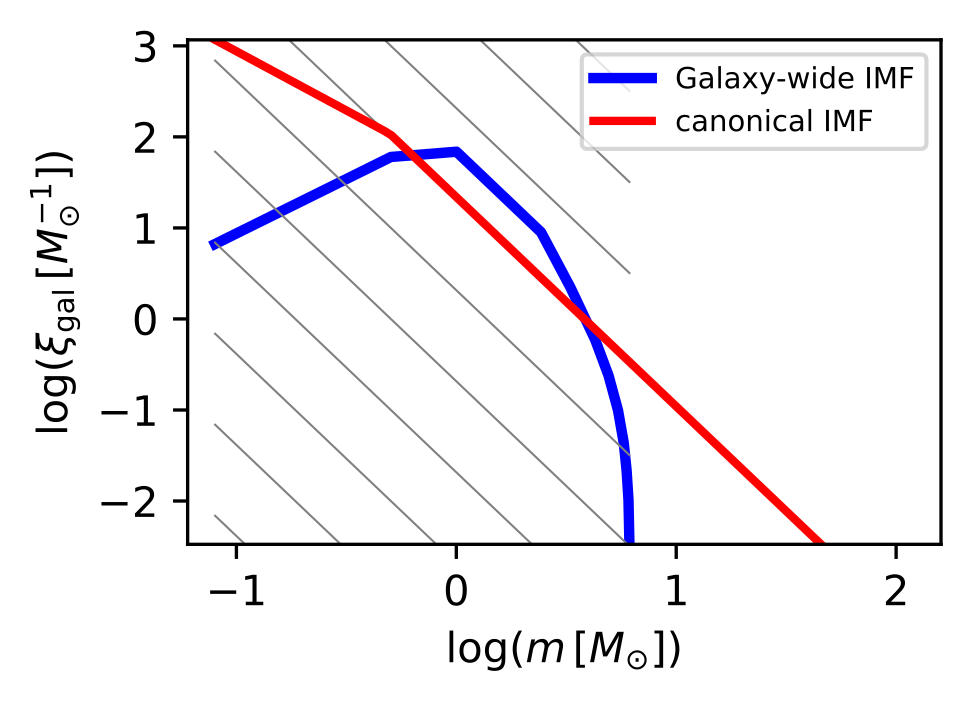
\includegraphics[width=\textwidth]{sfr1e-5-feh-5.png}
		\caption{SFR=$10^{-5}$, $[\frac{Fe}{H}]=-5$}
		\label{fig:2d-5dt}
	\end{subfigure}
	\caption{rebuild of A selection of IGIMF models which related to metalicity (in form of $[\frac{Fe}{H}$]=1,0,-3,-5)and SFR=$10^{-5},1,10^{4} \frac{M_{\odot}}{yr}$. All IMF models are
		normalized to the total stellar mass formed over $\delta t = 10 Myr$ to make the comparison with the canonical IMF (black dashed line in each panel)
		quantitative.}
	\label{fig:feh-5}
\end{figure}
\begin{figure}
	\centering
	\begin{subfigure}[b]{0.4\textwidth}
		%	\centering
		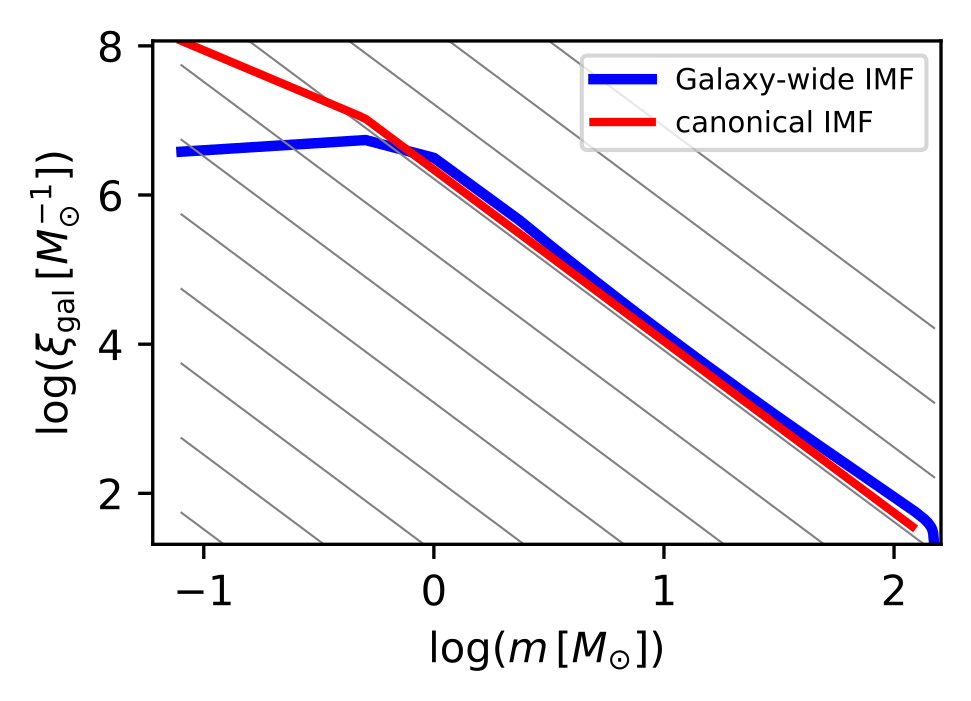
\includegraphics[width=\textwidth]{sfr1-feh-3.png}
		\caption{SFR=$10^{0}$, $[\frac{Fe}{H}]=-3$}
		\label{fig:s1e4-1}
	\end{subfigure}
	\begin{subfigure}[b]{0.4\textwidth}
		%\centering
		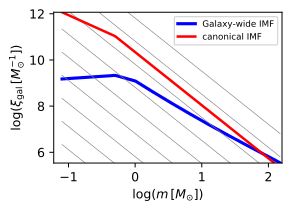
\includegraphics[width=\textwidth]{sfr1e4-feh-3.png}
		\caption{SFR=$10^{4}$, $[\frac{Fe}{H}]=-3$}
		\label{fig:2d-5dt}
	\end{subfigure}
	
	\begin{subfigure}[b]{0.45\textwidth}
		%\centering
		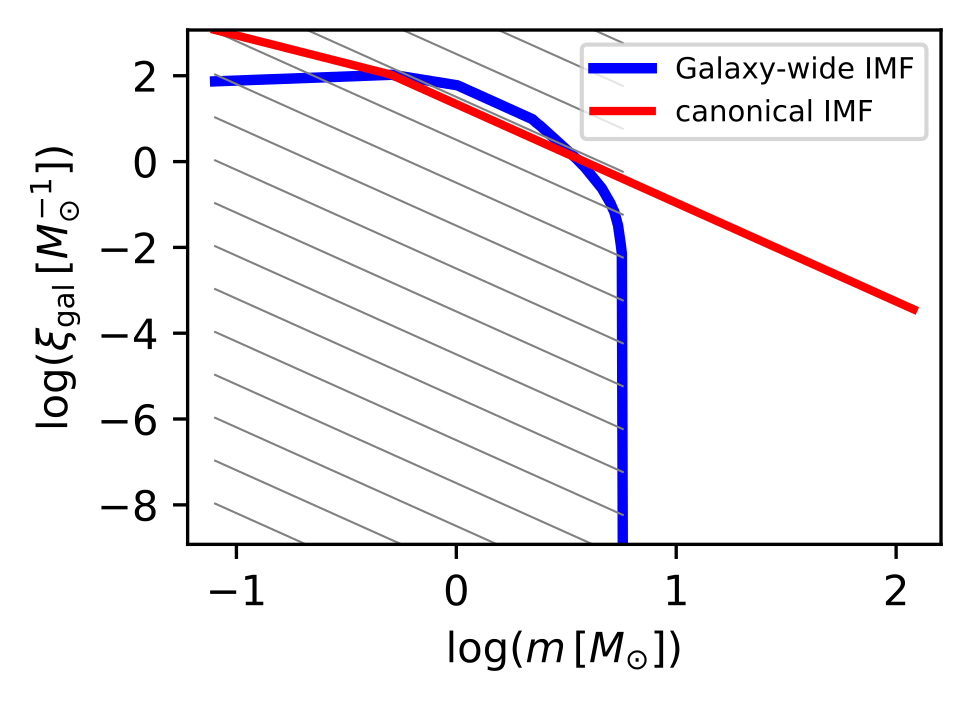
\includegraphics[width=\textwidth]{sfr1e-5-feh-3.png}
		\caption{SFR=$10^{-5}$, $[\frac{Fe}{H}]=-3$}
		\label{fig:2d-5dt}
	\end{subfigure}
	\caption{rebuild of A selection of IGIMF models which related to metalicity (in form of $[\frac{Fe}{H}$]=-3)and SFR=$10^{-5},1,10^{4} \frac{M_{\odot}}{yr}$. All IMF models are
		normalized to the total stellar mass formed over $\delta t = 10 Myr$ to make the comparison with the canonical IMF (black dashed line in each panel)
		quantitative.}
	\label{fig:feh-3}
\end{figure}

